%% abtex2-modelo-trabalho-academico.tex, v-1.9.2 laurocesar
%% Copyright 2012-2014 by abnTeX2 group at http://abntex2.googlecode.com/ 
%%
%% This work may be distributed and/or modified under the
%% conditions of the LaTeX Project Public License, either version 1.3
%% of this license or (at your option) any later version.
%% The latest version of this license is in
%%   http://www.latex-project.org/lppl.txt
%% and version 1.3 or later is part of all distributions of LaTeX
%% version 2005/12/01 or later.
%%
%% This work has the LPPL maintenance status `maintained'.
%% 
%% The Current Maintainer of this work is the abnTeX2 team, led
%% by Lauro César Araujo. Further information are available on 
%% http://abntex2.googlecode.com/
%%
%% This work consists of the files abntex2-modelo-trabalho-academico.tex,
%% abntex2-modelo-include-comandos and abntex2-modelo-references.bib
%%

% ------------------------------------------------------------------------
% ------------------------------------------------------------------------
% abnTeX2: Modelo de Trabalho Academico (tese de doutorado, dissertacao de
% mestrado e trabalhos monograficos em geral) em conformidade com 
% ABNT NBR 14724:2011: Informacao e documentacao - Trabalhos academicos -
% Apresentacao
% ------------------------------------------------------------------------
% ------------------------------------------------------------------------


\documentclass[
        % -- opções da classe memoir --
        12pt,                           % tamanho da fonte
        openright,                      % capítulos começam em pág ímpar (insere página vazia caso preciso)
        twoside,                        % para impressão em verso e anverso. Oposto a oneside
        a4paper,                        % tamanho do papel. 
        % -- opções da classe abntex2 --
        %chapter=TITLE,         % títulos de capítulos convertidos em letras maiúsculas
        %section=TITLE,         % títulos de seções convertidos em letras maiúsculas
        %subsection=TITLE,      % títulos de subseções convertidos em letras maiúsculas
        %subsubsection=TITLE,% títulos de subsubseções convertidos em letras maiúsculas
        % -- opções do pacote babel --
        english,                        % idioma adicional para hifenização
        french,                         % idioma adicional para hifenização
        spanish,                        % idioma adicional para hifenização
        brazil                          % o último idioma é o principal do documento
        ]{abntex2}

% ---
% Pacotes básicos 
% ---
\usepackage{lmodern}                    % Usa a fonte Latin Modern                      
\usepackage[T1]{fontenc}                % Selecao de codigos de fonte.
\usepackage[utf8]{inputenc}             % Codificacao do documento (conversão automática dos acentos)
\usepackage{lastpage}                   % Usado pela Ficha catalográfica
\usepackage{indentfirst}                % Indenta o primeiro parágrafo de cada seção.
\usepackage{color}                              % Controle das cores
\usepackage{graphicx}                   % Inclusão de gráficos
\usepackage{microtype}                  % para melhorias de justificação
% ---
                
% ---
% Pacotes adicionais, usados apenas no âmbito do Modelo Canônico do abnteX2
% ---
\usepackage{lipsum}                             % para geração de dummy text
% ---

% ---
% Pacotes de citações
% ---
\usepackage[brazilian,hyperpageref]{backref}     % Paginas com as citações na bibl
\usepackage[alf]{abntex2cite}                    % Citações padrão ABNT
\usepackage{lmodern}                             % Usa a fonte Latin Modern                      
\usepackage[T1]{fontenc}                         % Selecao de codigos de fonte.
\usepackage[utf8]{inputenc}                      % Codificacao do documento (conversão automática dos acentos)
\usepackage{lastpage}                            % Usado pela Ficha catalográfica
\usepackage{indentfirst}                         % Indenta o primeiro parágrafo de cada seção.
\usepackage{color}                               % Controle das cores
\usepackage{microtype}                           % para melhorias de justificação

% --- 
% CONFIGURAÇÕES DE PACOTES
% --- 

% ---
% Configurações do pacote backref
% Usado sem a opção hyperpageref de backref
\renewcommand{\backrefpagesname}{Citado na(s) página(s):~}
% Texto padrão antes do número das páginas
\renewcommand{\backref}{}
% Define os textos da citação
\renewcommand*{\backrefalt}[4]{
        \ifcase #1 %
                Nenhuma citação no texto.%
        \or
                Citado na página #2.%
        \else
                Citado #1 vezes nas páginas #2.%
        \fi}%

\usepackage{amsmath, amssymb, amscd, amsthm, amsfonts}
\usepackage{bm}
\usepackage{graphicx}
\usepackage{hyperref}

\usepackage{tikz}
\usepackage{pgfplots}
\usepackage{tabto}
\usepackage[siunitx]{circuitikz}
\usetikzlibrary{patterns, arrows, calc, decorations}
\usetikzlibrary{decorations.markings}
\usetikzlibrary{decorations.text}
\usepackage{hyperref}
\hypersetup{
  colorlinks=true,linkcolor=blue,urlcolor=cyan
}
% \usepackage[portuguese]{babel} % Corrige linguaagem
\usepackage{svg}

\title{Eletro\'im\~as e suas aplicaç\~oes}
\author{Juan Vasconcelos, Matrícula: 201907140019 \and Jo\~ao Pedro Albuquerque, Matrícula: 201907140017 \and Jo\~ao Paulo de Andrade, Matrícula: 201907140009 \and Thiago Toni, Matrícula: 201907140061}
\date{}


\instituicao{%
  Universidade Federal do Pará
  \par
  Faculdade de Engenharia Elétrica e Biomédica
  }
\tipotrabalho{Trabalho Acadêmico}

\makeatletter
\hypersetup{
        %pagebackref=true,
                pdftitle={\@title}, 
                pdfauthor={\@author},
                pdfsubject={\imprimirpreambulo},
                pdfcreator={LaTeX with abnTeX2},
                pdfkeywords={abnt}{latex}{abntex}{abntex2}{trabalho acadêmico}, 
                colorlinks=true,                % false: boxed links; true: colored links
                linkcolor=blue,                 % color of internal links
                citecolor=blue,                 % color of links to bibliography
                filecolor=magenta,                      % color of file links
                urlcolor=blue,
                bookmarksdepth=4
}
\makeatother

\begin{document}

\frenchspacing 

\imprimircapa

\imprimirfolhaderosto*


% ---
% inserir lista de ilustrações
% ---
\pdfbookmark[0]{\listfigurename}{lof}
\listoffigures*
\cleardoublepage
% ---

% ---
% inserir o sumario
% ---
\pdfbookmark[0]{\contentsname}{toc}
\tableofcontents*
\cleardoublepage
% ---

% \tableofcontents

\part{Introdução}
\chapter[Contexto Histórico]{Contexto Histórico}

\section{A Invenção do Eletroímã}\label{chap:introdução}
Eletroímãs estão presentes desde 1824 com a invenção de Hans Christian Ørsted após
sua descorberta de 1820 onde descreve que a corrente elétrica de um fio deflete 
uma bússola. Sua invenção, presente na figura~\ref{fig:chap:introdução:1},
consistia de um pedaço de ferro maciço em formato de ferradura de cavalo envolvido
por um condutor

\begin{figure}[htp]
  \centering
  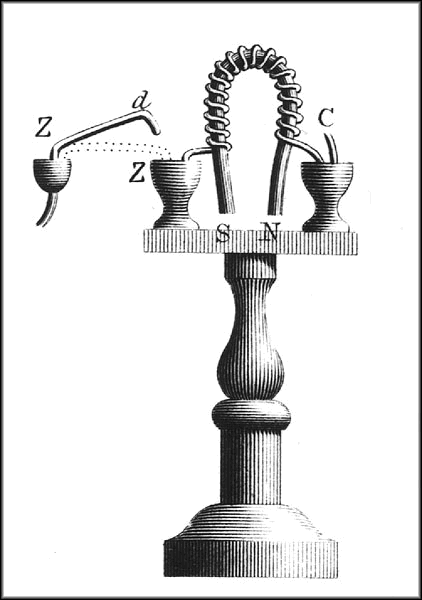
\includegraphics[width=0.2\columnwidth]{Sturgeon_electromagnet.png}
  \label{fig:chap:introdução:1}
  \caption{Eletroímã inventado por Ørsted}
\end{figure}


\part{Desenvolvimento}
\chapter[Embasamento Matemático]{Embasamento Matemático}\label{chap:embasamento}
\section{Indução Magnética e a Lei de Ampère}
O princípio de funcionamento de eletroímãs advem da Lei de Ampère:
\begin{gather}
  \underbrace{ \oint_{\partial \Sigma} \bm{B} \cdot \: d{\bm{l}} }_\text{ campo magnético } = \mu_0 \left( \underbrace{ \iint_{\Sigma} \bm{J} \cdot \: d{\bm{S}} }_\text{corrente} + \underbrace{ \varepsilon \dfrac{d}{dt} \iint_{\Sigma} \bm{E} \: d{\bm{S}} }_\text{componente variante no tempo}  \right)
\end{gather}
ou igualmente em sua forma diferencial:
\begin{gather}
  \underbrace{\nabla \times \bm{B}}_\text{campo magnético} = \mu_0 \left( \underbrace{\bm{J}}_\text{corrente} + \underbrace{\varepsilon \dfrac{\partial \bm{E}}{\partial t}}_\text{componente variante no tempo} \right) 
\end{gather}

Ignorando por hora a componente variante no tempo, podemos nos focar no resultado
interessante para máquinas assíncronas: corrente elétrica em um condutor gera um
campo magnético, como ilustrado na figura~\ref{fig:chap:embasamento:1}. Enrolando
um condutor em forma helicoidal (um solenóide), que equivale a alinhar anéis em
sequência, teremos uma amplificação do campo, devido à contribuição de cada porção
de corrente no condutor, como ilustrado na figura~\ref{fig:chap:embasamento:2}.

\begin{figure}[htp]
  \centering
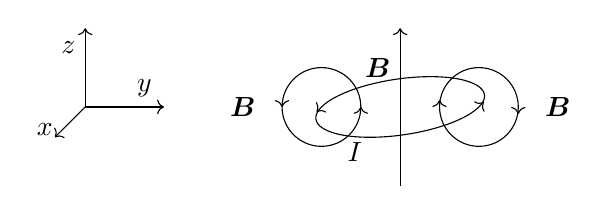
\begin{tikzpicture}
  % anel com corrente
  \draw[
    decoration={markings, mark=at position 0 with {\arrow{<}}},
    decoration={markings, mark=at position 0.5 with {\arrow{<}}},
    postaction={decorate}
    ] (0,0,0) [y={(0,0,1)}] circle (1) node[above left] {};
  \node at (0,1.5,0) [y={(0,0,1)}] {$I$};
  
  % Campo magnético
  \draw[
    decoration={markings, mark=at position 0 with {\arrow{<}}},
    decoration={markings, mark=at position 0.5 with {\arrow{<}}},
    postaction={decorate}
    ] (1,0,0) [y={(0,1,0)}] circle (0.5);
  \node at (2,0,0) [y={(0,1,0)}] {$\bm{B}$};
  \draw[
    decoration={markings, mark=at position 0 with {\arrow{>}}},
    decoration={markings, mark=at position 0.5 with {\arrow{>}}},
    postaction={decorate}
    ] (-1,0,0) [y={(0,1,0)}] circle(0.5);
  \node at (-2,0,0) [y={(0,1,0)}] {$\bm{B}$};
  \draw[->] (0,-1,0) [y={(0,1,0)}] -- ++(0,2,0) node[left, near end]{$\bm{B}$};


  \draw[->] (-4,0,0) [y={(0,1,0)}] -- ++(0,1,0) node[left, near end]{$z$};
  \draw[->] (-4,0,0) [y={(0,0,1)}] -- ++(0,1,0) node[left, near end]{$x$};
  \draw[->] (-4,0,0) [y={(0,0,1)}] -- ++(1,0,0) node[above, near end]{$y$};
\end{tikzpicture}
\caption{Campo magnético atravessando um anel com corrente anti-horária}
\label{fig:chap:embasamento:1}
\end{figure}

\begin{figure}[htp]
  \centering
  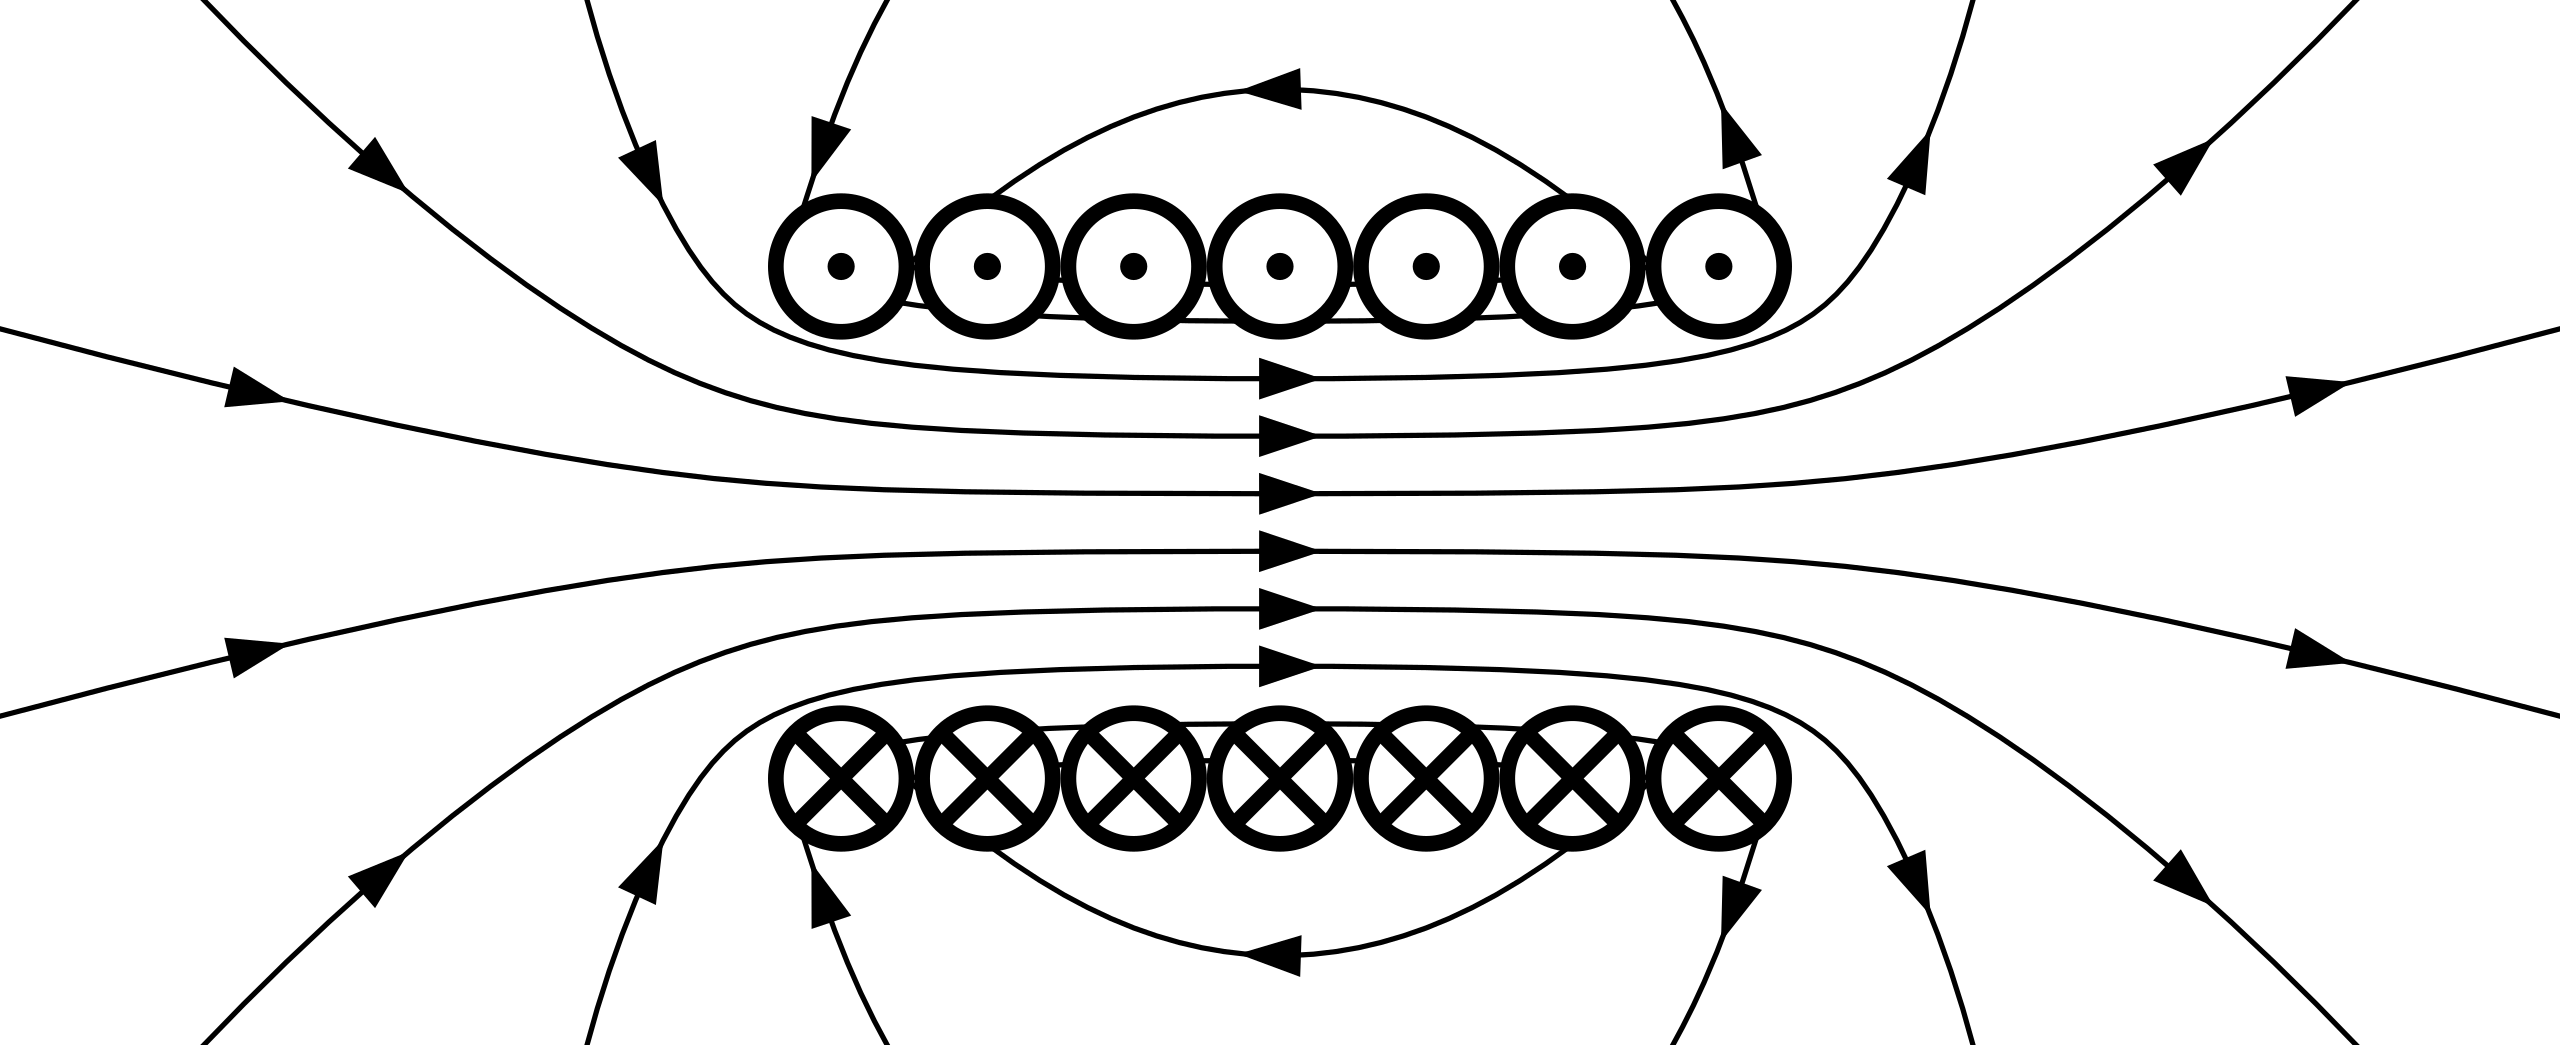
\includegraphics[width=0.5\columnwidth]{2560px-VFPt_Solenoid_correct2.svg.png}
  \caption{Campo magnético dentro de um solenóide}
  \label{fig:chap:embasamento:2}
\end{figure}

\begin{figure}[htp]
  \centering
  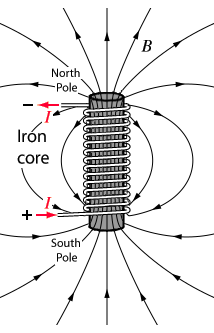
\includegraphics[width=0.2\columnwidth]{Elecmagnet.png}
  \caption{Solenoide amplificando o campo magnético no núcleo}
  \label{fig:chap:embasamento:3}
\end{figure}


\end{document}
